\documentclass{standalone}
\usepackage{tikz}
\usetikzlibrary{shapes.geometric, arrows.meta, positioning}

\begin{document}

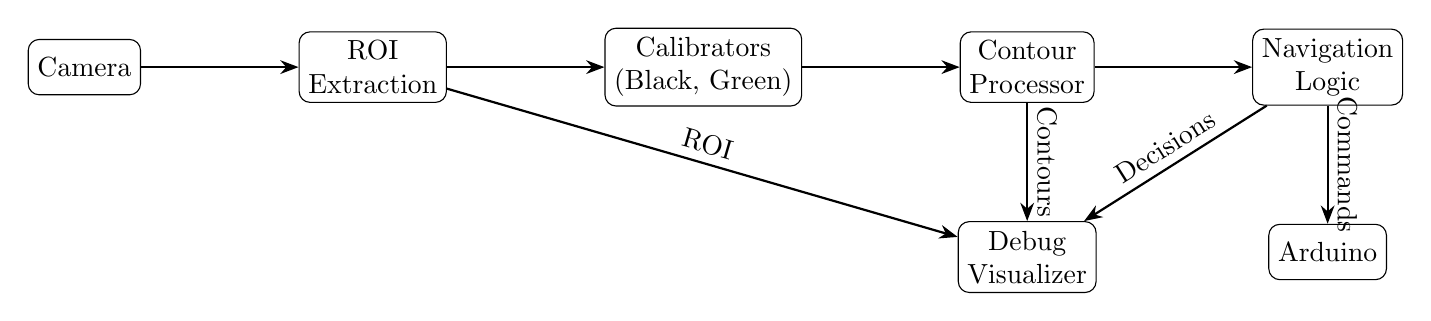
\begin{tikzpicture}[
    box/.style={rectangle, draw, rounded corners, minimum height=2em, minimum width=4em, align=center},
    arrow/.style={-Stealth, thick},
    node distance=1.5cm and 2cm
]

% Nodes
\node[box] (camera) {Camera};
\node[box, right=of camera] (roi) {ROI\\Extraction};
\node[box, right=of roi] (calib) {Calibrators\\(Black, Green)};
\node[box, right=of calib] (contour) {Contour\\Processor};
\node[box, right=of contour] (nav) {Navigation\\Logic};
\node[box, below=of nav] (arduino) {Arduino};
\node[box, below=of contour] (debug) {Debug\\Visualizer};

% Arrows
\draw[arrow] (camera) -- (roi);
\draw[arrow] (roi) -- (calib);
\draw[arrow] (calib) -- (contour);
\draw[arrow] (contour) -- (nav);
\draw[arrow] (nav) -- (arduino) node[midway, above, sloped] {Commands};
\draw[arrow] (contour) -- (debug) node[midway, above, sloped] {Contours};
\draw[arrow] (nav) -- (debug) node[midway, above, sloped] {Decisions};
\draw[arrow] (roi) -- (debug) node[midway, above, sloped] {ROI};

\end{tikzpicture}

\end{document}